\chapter{Implementácia}
- Programovacie jazyky a knižnice: 
	C, esp-idf v4.0, esp-dsp v1.2.0, MPack v1.1 (\url{https://ludocode.github.io/mpack/md_docs_expect.html}), FreeRTOS v9.0.0
- Python3.10, numpy, scipy (stats, signal, fft, interpolate), pandas, seaborn, matplotlib
- msgpack, json, cmd


\begin{figure}[h]
\centering
\begin{subfigure}[b]{0.65\textwidth}
    \centering
    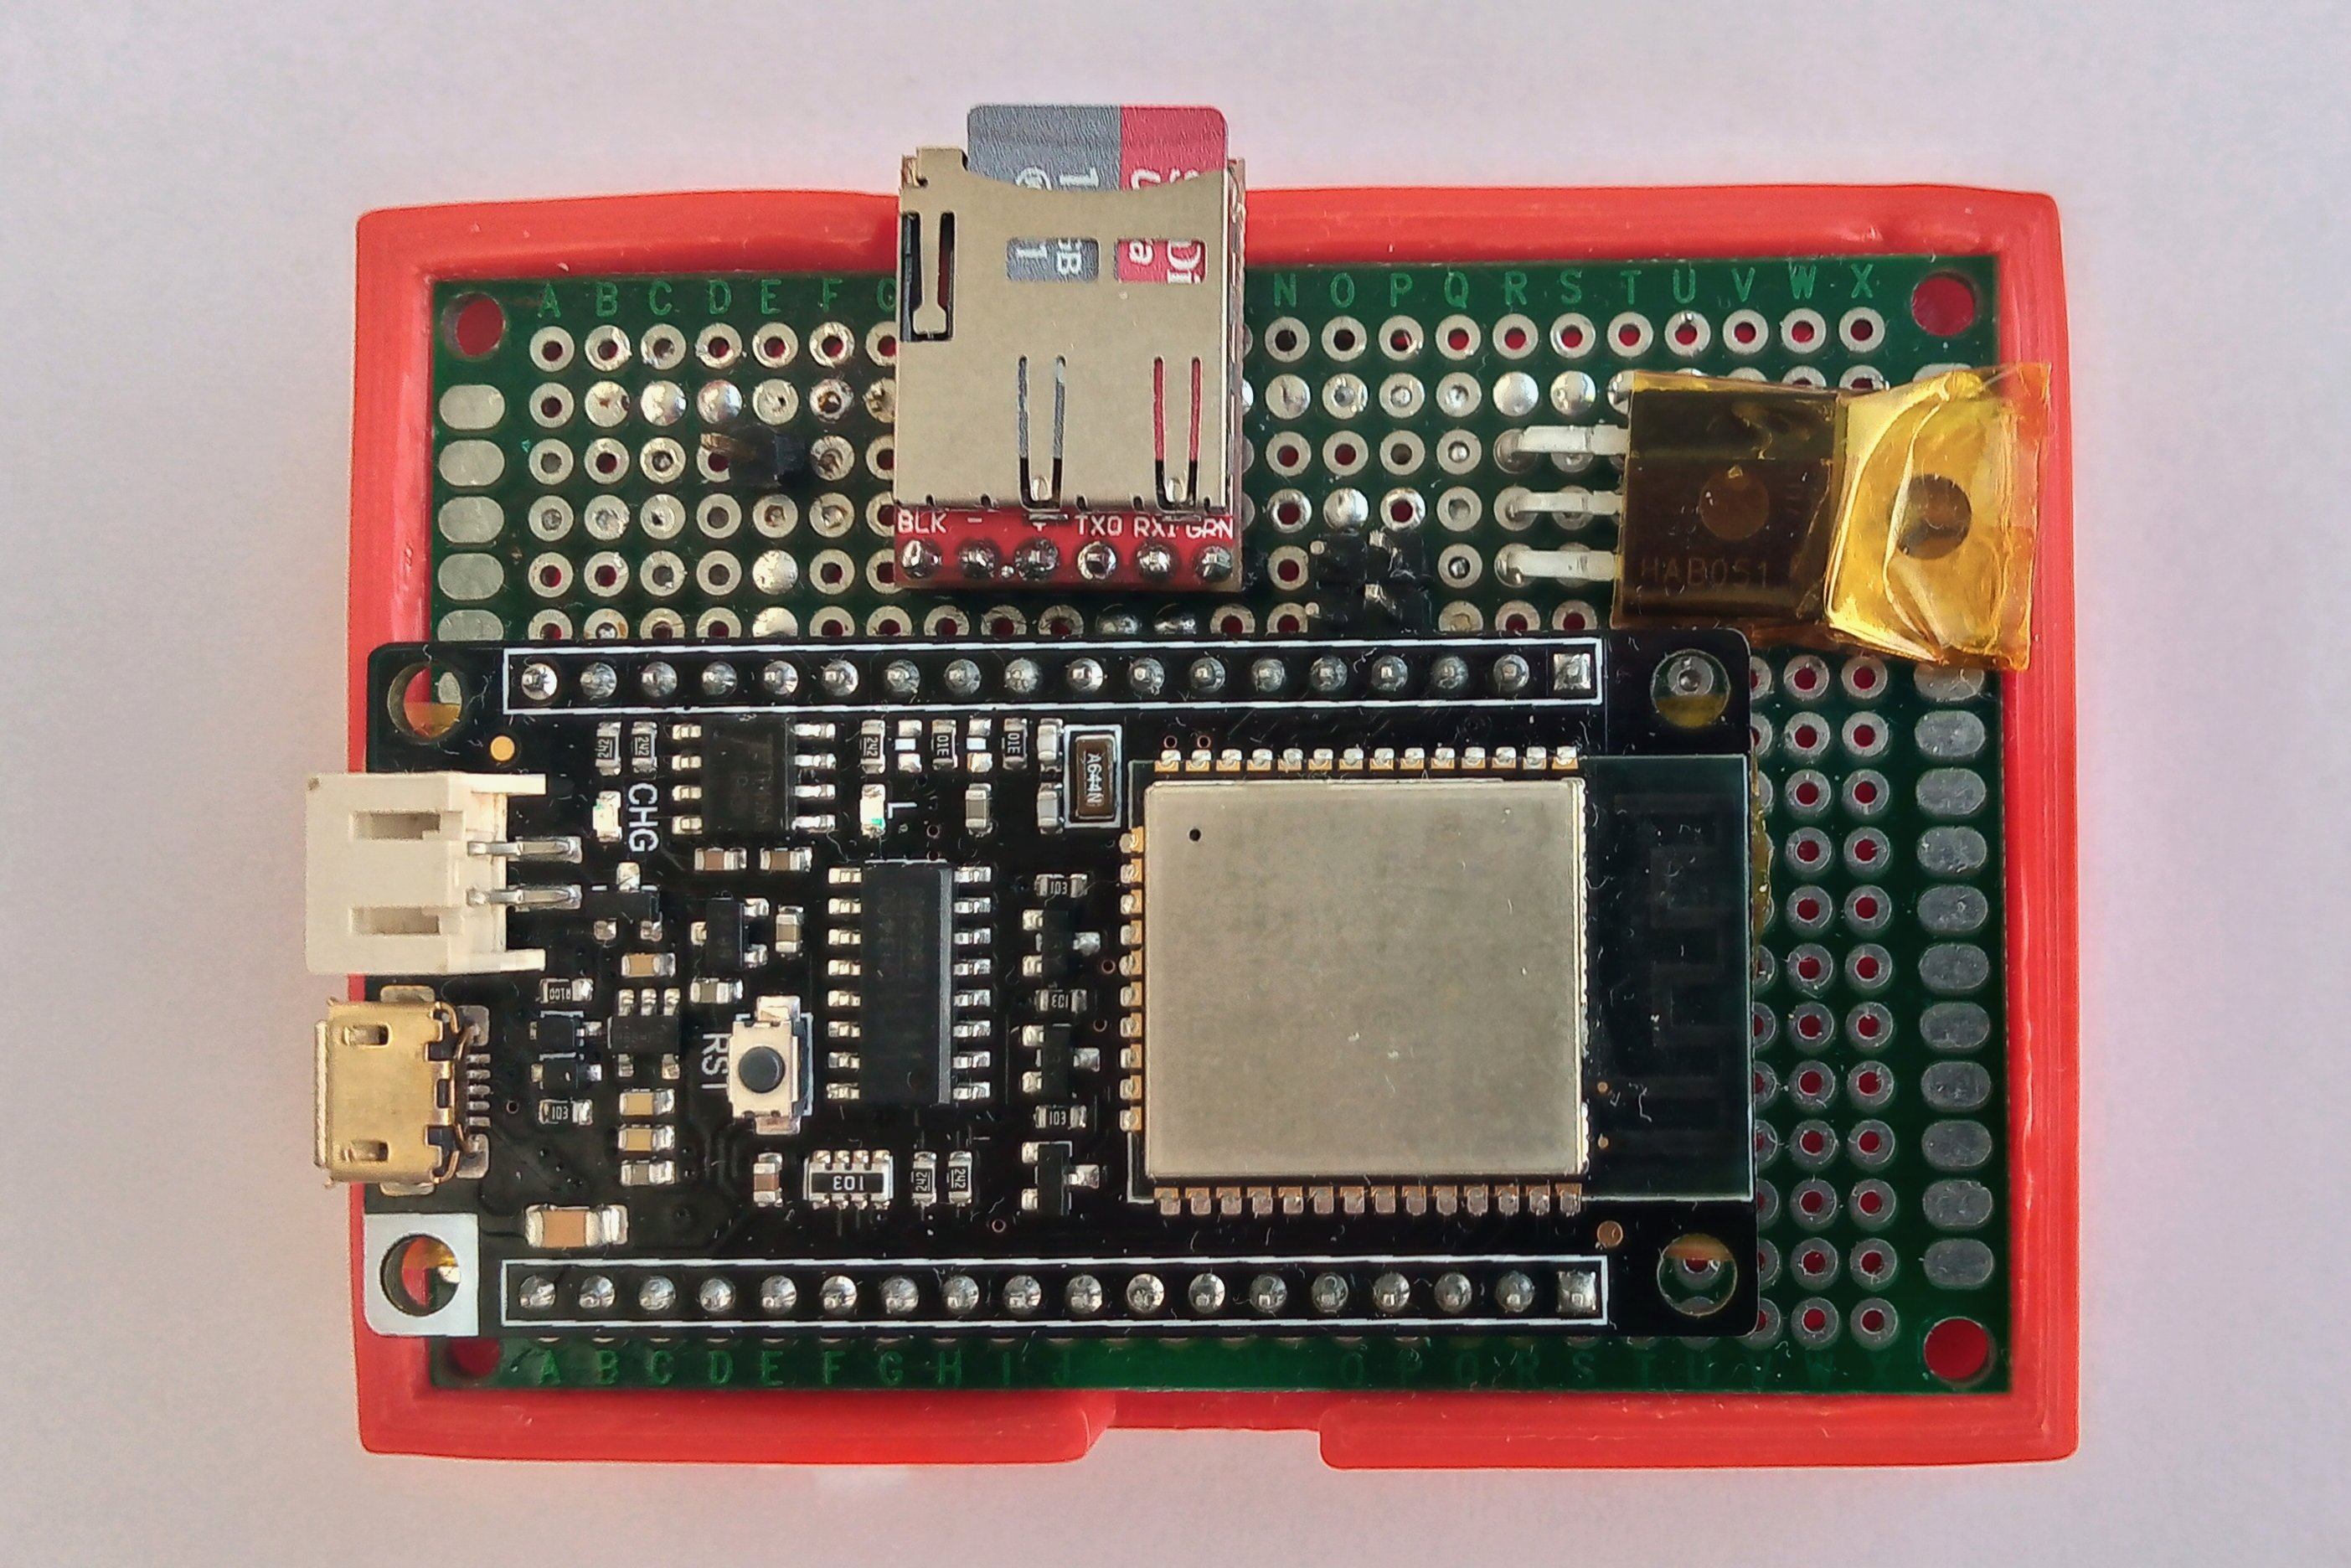
\includegraphics[width=\textwidth]{figures/design/esp32.jpg}
\end{subfigure}
\hfill
\begin{subfigure}[b]{0.3\textwidth}
    \centering
    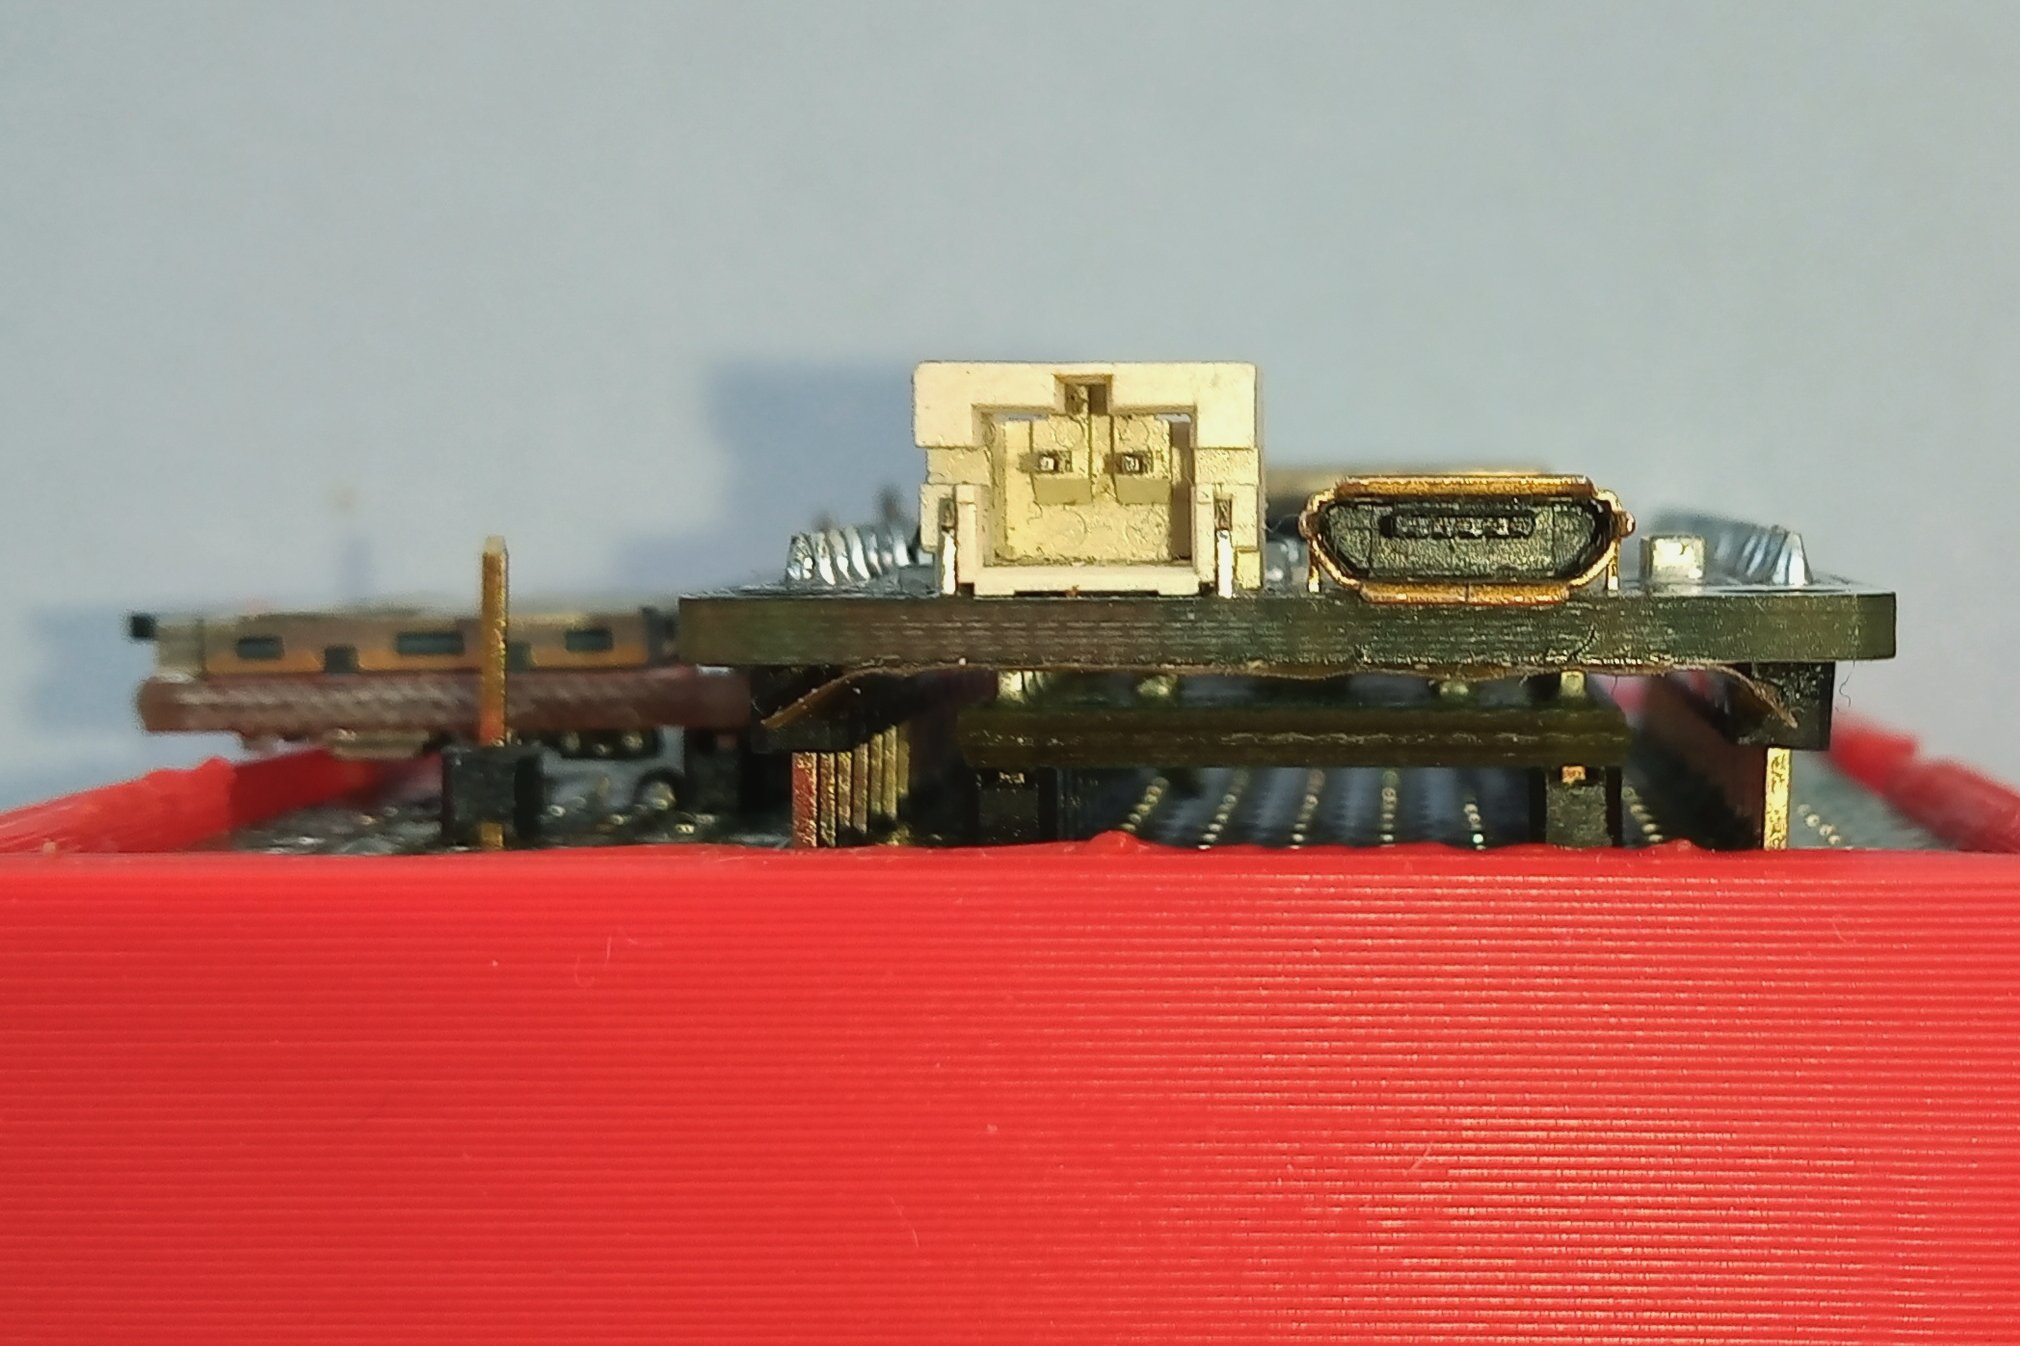
\includegraphics[width=\textwidth]{figures/design/esp32-front.jpg}
\end{subfigure}
\label{schematics}
\caption{Schéma zapojenia hardvéru}
\end{figure}

\section{Adaptér akcelerometra}
Načítavanie a prepočet osi zrýchlenia z akcelerometra % na m/s^2 vo funkcii imu\_acceleration (imu, *x)
Nastavenie vzorkovacej frekvencie a dynamického rozsahu

\begin{lstlisting}[style=cstyle]
uint8_t buffer[6];
spi_read_buffer(imu->dev, 0x80 | IMU_OUT_X_L_XL, 6, buffer);
    
uint8_t xlo = buffer[0];
int16_t xhi = buffer[1];
xhi = (xhi << 8) | xlo;
*x = xhi * imu->precision * G_CONSTANT;
\end{lstlisting}


\section{Frekvenčná transformácia}
Uprava DCT v knižnici
\begin{lstlisting}[style=cstyle,caption=Transformácia do frekvenčnej domény vo funkcii process\_spectrum]
for (uint16_t i = 0; i < n; i++) {
	spectrum[2*i+0] = buffer[i] * window[i];
    spectrum[2*i+1] = 0;
}
dsps_fft2r_fc32_ae32(spectrum, n);
dsps_bit_rev2r_fc32(spectrum, n);
dsps_cplx2reC_fc32(spectrum, n);
\end{lstlisting}
 
Magnituda spektra v dB
\begin{lstlisting} [style=cstyle]         
for (uint16_t i = 0; i < bins; i++)
	spectrum[i] = dsps_sqrtf_f32_ansi(
          square(spectrum[i*2]) + square(spectrum[i*2+1])
    );

float ref = maximum(spectrum, bins);
for (uint16_t i = 0; i < bins; i++)
	spectrum[i] = 20 * log10f(spectrum[i] / ref);
\end{lstlisting}


\section{Detekcia udalostí}
\begin{lstlisting}[style=cstyle]
typedef struct {
    SpectrumEventAction action;
    uint32_t start;
    uint32_t duration;
    int32_t last_seen;
    float amplitude;
} SpectrumEvent;
\end{lstlisting}

\section{Vzdialená konfigurácia}
- Nástroj klienta
- Opis štruktúr konfigurácie
- Uloženie v pamäti
\begin{lstlisting}[style=cstyle]
typedef struct {
    SamplingConfig sensor;
    SmoothingConfig tsmooth;
    StatisticsConfig stats;
    FFTTransformConfig transform;
    SmoothingConfig fsmooth;
    EventDetectionConfig peak;
    SaveFormatConfig logger;
} Configuration;
\end{lstlisting}
- MessagePack formát - serilizácia a deserializácia (výmena iba pri zmene)

\begin{lstlisting}[style=cstyle]
Configuration c;
memcpy(&c, &conf, sizeof(c));
change = config_parse(event->data, event->data_len, &c, &error);

if (error) {
    esp_mqtt_client_publish(client, MQTT_TOPIC_SYSLOG, "config malformed", 0, 1, 0);
} else if (change) {
	nvs_save_config(&c);
	esp_mqtt_client_publish(client, MQTT_TOPIC_SYSLOG, "config applied", 0, 1, 0);
	esp_wifi_stop();
	esp_wifi_deinit();
	esp_restart();
}
\end{lstlisting}

\begin{verbatim}
# /etc/mosquitto/mosquitto.conf
listener 1883 0.0.0.0
allow_anonymous true
\end{verbatim}

\emptypage
